% Tabela: Recomendacoes ECC
\begin{table}[H]
	\centering
	\caption{FIPS PUB 186-4 \cite{nist2013fipspub186}: Recomendação para ECC sobre P-256.}
	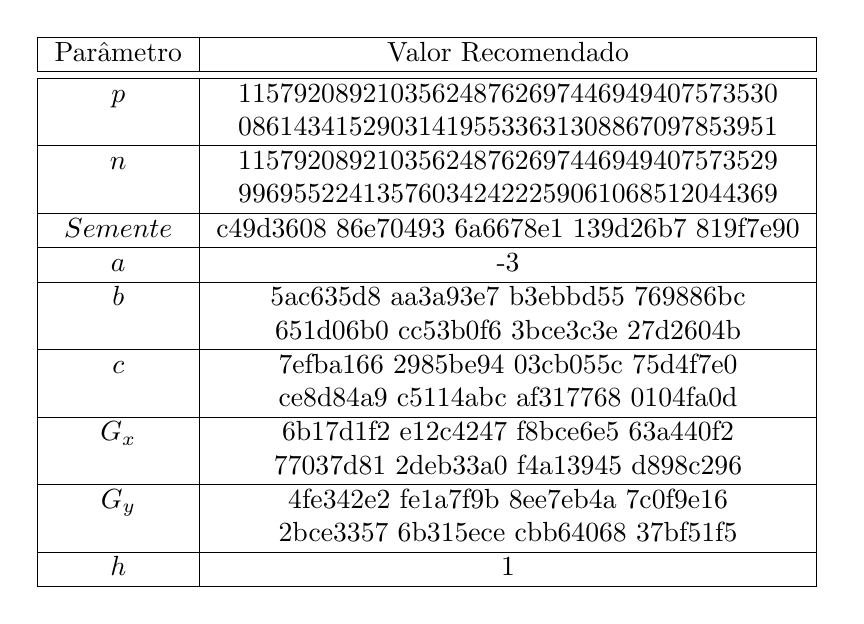
\begin{tikzpicture}

		\node[thick, align=center] (table) {
			\begin{tabular}{ |c|c| }
				\hline
				% \multicolumn{2}{ |c| }{Recomendações para ECC sobre P-256} \\
				% \hline \hline
				Parâmetro & Valor Recomendado \\
				\hline \hline
				$p$       & 115792089210356248762697446949407573530 \\
				          & 086143415290314195533631308867097853951 \\
				\hline
				
				$n$       & 115792089210356248762697446949407573529 \\
				          & 996955224135760342422259061068512044369 \\
				\hline
				
				$Semente$ & c49d3608 86e70493 6a6678e1 139d26b7 819f7e90 \\
				\hline
				
				$a$       & -3 \\
			    \hline
			    
				$b$       & 5ac635d8 aa3a93e7 b3ebbd55 769886bc \\
				          & 651d06b0 cc53b0f6 3bce3c3e 27d2604b \\
				\hline
				
				$c$       & 7efba166 2985be94 03cb055c 75d4f7e0 \\
				          & ce8d84a9 c5114abc af317768 0104fa0d \\
				\hline
				
				$G_{x}$   & 6b17d1f2 e12c4247 f8bce6e5 63a440f2 \\
				          & 77037d81 2deb33a0 f4a13945 d898c296 \\
				\hline
				
				$G_{y}$   & 4fe342e2 fe1a7f9b 8ee7eb4a 7c0f9e16 \\
				          & 2bce3357 6b315ece cbb64068 37bf51f5 \\
				\hline
				
				$h$       & 1 \\
			    \hline
			\end{tabular}
		};

	\end{tikzpicture}
	\label{tab:recomendacoes_ecc}
\end{table}